% !TEX TS-program = xelatex
% !TEX encoding = UTF-8 Unicode

% \documentclass[AutoFakeBold]{LZUThesis}
\documentclass[AutoFakeBold]{LZUThesis}

\begin{document}
%=====%
%
%封皮页填写内容
%
%=====%

% 标题样式 使用 \title{{}}; 使用时必须保证至少两个外侧括号
%  如: 短标题 \title{{第一行}},  
% 	      长标题 \title{{第一行}{第二行}}
%             超长标题\tiitle{{第一行}{...}{第N行}}

\title{{利用机器学习进行气体探测器}{径迹重建的算法研究}}



% 标题样式 使用 \entitle{{}}; 使用时必须保证至少两个外侧括号
%  如: 短标题 \entitle{{First row}},  
% 	      长标题 \entitle{{First row}{ Second row}}
%             超长标题\entitle{{First row}{...}{ Next N row}}
% 注意:  英文标题多行时 需要在开头加个空格 防止摘要标题处英语单词粘连。
\entitle{
    {Research on Algorithms of Using Machine Learning}
    {to Reconstruct the Tracks in Gas Detectors}
}

\author{王文军}
\major{放射化学}
\advisor{张毅}
\college{核科学与技术学院}
\grade{2017级}



\maketitle

%==============================%
% ↓ ↓ ↓ 诚信说明页 授权说明书
%==============================%

% 1. 可以调整签字的宽度,现在是40
% 2. 去掉raisebox的相关注释(注意上下大括号对应),可以改变-5那个数字调整签名和横线的上下位置

% % 你的签名,signature.pdf 改为你的签名文件名,
% \mysignature{
%     % \raisebox{-5pt}{
%         \includegraphics[width=40pt]{signature.pdf}
%     % }
% }
% % 你手写的日期,signature.pdf 改为你的手写的日期文件名
% \mytime{
%     % \raisebox{-5pt}{
%         \includegraphics[width=40pt]{signature.pdf}
%     % }
% }
% % 老师的手写签名,signature.pdf 改为老师的手写签名文件名
% \supervisorsignature{
%     % \raisebox{-5pt}{
%         \includegraphics[width=40pt]{signature.pdf}
%     % }
% }
% % 老师手写的时间,signature.pdf 改为老师的手写的日期文件名
% \teachertime{
%     % \raisebox{-5pSt}{
%         \includegraphics[width=40pt]{signature.pdf}
%     % }
% }
% % 老师手写的成绩
% \recommendedgrade{
%     % \raisebox{-5pt}{
%         \includegraphics[width=40pt]{signature.pdf}
%     % }
% }

\makestatement

%==============================%
% ↑ ↑ ↑ 诚信说明页 授权说明书
%==============================%


%=====%
%论文(设计)成绩:注意2007的模板要求,成绩页在最后,2021要求成绩页在摘要前面
%=====%

% % 下面这些注释掉可以去掉成绩、评语什么的
% \supervisorcomment{导师评价你人很好}


% \committeecomment{优秀}

% \finalgrade{100}
% % 上面这些注释掉可以去掉成绩、评语什么的

\Grade %这一句才是成绩页,上面是填写


\frontmatter



%英文摘要
\EnAbstract{\fontspec{Times New Roman} {}
The technique of Time Projection Chamber (TPC) is more and more employed in the experimental research of nuclear fission due to several advantages such as solid angle, energy resolution, and correlated measurement of multi observables. 

In this paper, based on U-235 fission data generated by simulation, using software such as Srim, Garfield++, etc., I completed the track reconstruction of U-235 fission fragments under the time projection chamber.
And based on the track reconstruction data, with the help of the unique advantages of the artificial neural network algorithm that does not rely on specific mathematical expressions, a brand-new fission fragment track analysis technology is established, and a fission fragment nuclide classification model is realized.
}
{time projection chamber; fission products measurement; artificial neural network; classification
}



%中文摘要
\ZhAbstract{
时间投影室 (Time Projection Chamber, TPC) 技术因其在立体角、能量分辨以及多观测量关联测量等方面的显著优势而越来越多地应用于原子核裂变的实验研究中。

本论文基于模拟计算生成的 U-235 裂变数据,利用 Srim, Garfield++ 等软件,完成了 U-235 裂变碎片于时间投影室下的径迹重建。并且基于径迹重建数据,借助人工神经网路算法不依赖于具体数学表达形式的独特优势,建立全新的裂变碎片径迹分析技术,实现了裂变碎片核素分类模型。
}
{
时间投影室; 裂变产物测量; 人工神经网络;核素分类
}



%生成目录
\tableofcontents
\thispagestyle{empty}


%文章主体
\mainmatter

\chapter{绪 \qquad 论}
\section{研究背景}
自从 1938 年发现原子核裂变以来\cite{meitner1939disintegration},人们就一直没有停止过对该领域的研究。
在原子核裂变中,一个原子核受到激发,然后分裂成多个碎片。裂变碎片通常为两个较轻的原子核,但是在极少数情况下也有可能分裂为三个较轻的原子核\cite{vijayaraghavan2014collinear}。
在某些情况下,原子核裂变这一过程可能是自发发生的,也可能是通过某些粒子诱导受激发的原子核发生的。例如:中子、质子、氘核、$\alpha$ 粒子或者是具有 $\gamma$ 射线形式的电磁辐射。
与此同时,原子核裂变会释放出大量能量,形成具有放射性的产物,同时发射出多个中子和光子。
这些中子可以在可裂变物质的附近原子核中引起裂变,并释放出更多的中子,这些中子可以重复该过程,从而导致链反应,其中大量原子核发生裂变并释放出大量能量\cite{anderson1939neutron, bohr1939mechanism}。中子诱发的原子核裂变是中子与原子核碰撞并被吸收,从而使原子核受激发并分裂成碎片的过程。如果这些碎片(子核)不稳定或受激发,也可能分裂成更多碎片(图 \ref{fig_nuclear_fission})。 

\begin{figure}[H]
    \centering
    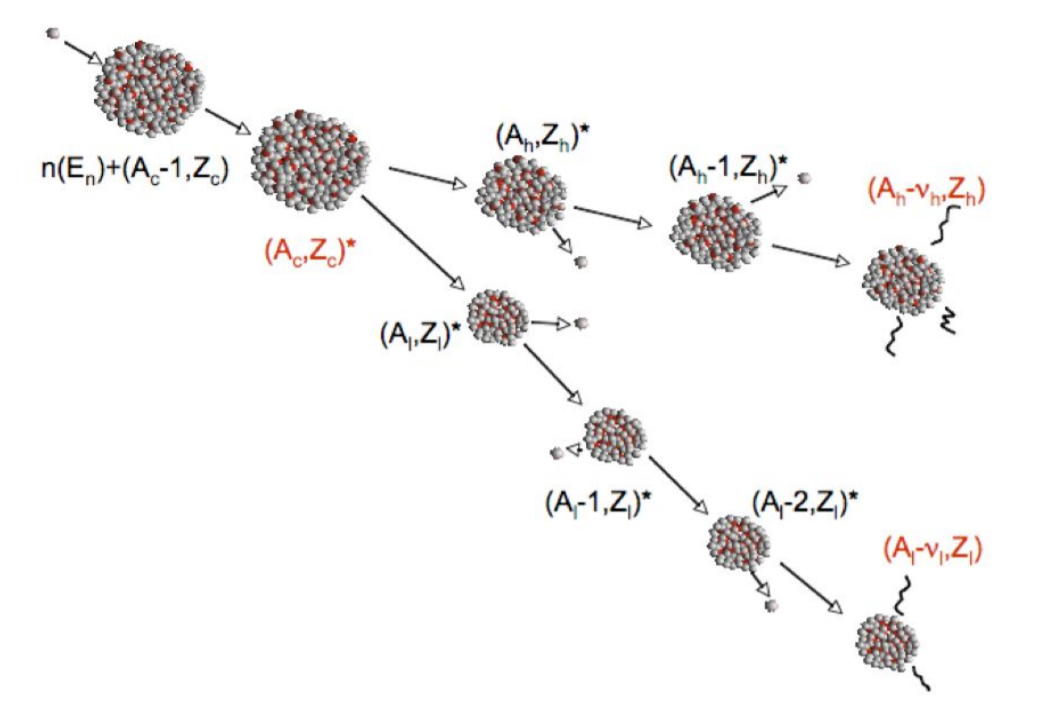
\includegraphics[width=0.7\textwidth]{figures/nuclear_fission.png}
    \caption{原子核裂变反应示意图\cite{kovacs1970angular}}
    \label{fig_nuclear_fission}
\end{figure}

现在,对原子核裂变的研究给能量、军事和核医学等领域带来了深刻的影响。核裂变已广泛地用于核武器和核反应堆等方向。核反应堆是可控的核反应,平均而言,在每个裂变期间发射的中子只会引起另一个裂变。而核武器是不受控制的裂变,裂变发射的中子会引起多核的裂变。近年来,由于对核裂变的进一步研究和开发,其逐渐广泛用于核素合成和天体物理学领域。

尽管自原子核裂变发现以来,人们一直在不断地进行研究,但是核裂变深层次地物理学仍然存在许多悬而未决的问题。
核裂变过程是一个高度复杂的多体量子力学问题,裂变路径上原子核的动力学难以计算,经过 75 年的裂变研究,如果想要完全理解这一过程,仍有很多被探索发现。

由于不存在适用于任意原子核的准确模型,因此必须测量许多原子核及其相关的特性,例如质量、半衰期、原子核结构等都是重要的参数。这些参数不仅可以帮助我们更好地理解原子核本身,还可以让我们理解它们在宏观尺度上是如何被创造地。毫无疑问,没有原子核裂变、衰变和许多其他核现象的详细模型,我们就无法理解恒星和大型宇宙学事件深层测究竟发生了什么。
除此之外,核数据在核能和国防应用中起着至关重要的作用,核物理研究很大程度上依赖于计算机软件仿真和建模,因此也依赖于实际可用的数据及其数据的不确定性。
因此,通过提供新的原子核裂变数据和中子诱发核反应的分析,将有助于我们更好地理解那些尚未通过实验充分验证的理论和模型\cite{bohr1939mechanism}。





\section{传统中子诱发核裂变测量技术}
对于由低能中子引起的原子核裂变,除瞬发的轻粒子之外,大多数裂变碎片是两个中等质量的重离子。
传统的裂变碎片观测方法分为物理方法和放射化学方法。
对于长寿命碎片,放射化学方法可以提供最准确的质量分布和电荷分布的测量结果,但在大多数情况下,放射化学方法仅限于对累积产率的测量。
对于短寿命碎片和多观测量,尤其是运动学观测的关联测量,化学方法在此方向上行不通。
物理方法主要包括双能量法、双速度法和能量动量法。双能量法利用裂变前后的动量守恒,通过测量两个碎片的动能比来确定两个碎片的质量。双能量法的优点是探测效率高,但对碎片电荷分布作用影响有限。同时,高精度的质量测量对靶材的制备过程也有很高的要求。双速度法的原理类似于双能量法,它可以以相对较低的检测效率为代价,更精确地测量碎片的质量。能量动量法主要使用电磁波谱仪,同时测量裂变碎片的能量和动量,然后计算裂变碎片的质量和电荷。能量动量法中碎片质量的测量精度可以与放射化学方法的结果相媲美,但检测效率不高,仅限于高产量碎片的测量。总的来说,与裂变碎片的质量相比,核电荷的实验测量更加困难。






\section{基于裂变时间投影室的新型核裂变测量技术}
David Nygren 在 1970 年代后期发明的时间投影室(Time Projection Chamber, TPC)是现在许多粒子和核物理实验中带电粒子径迹分析的基础\cite{nygren1978time}。
最初设计的时间投影室,可以允许在电子-正负电子对撞机上完全重建多达 20 个粒子的事件。
时间投影室是一种粒子检测器,能够对通过检测器介质传播的带电粒子进行完整的三维重建。在时间投影室中,均匀电场作用下,带电粒子穿过室腔时会沿着漂移轨迹上产生电子/离子对,电子在漂移区均匀电场作用下向读出板上移动,之后通过记录读出板上的信号幅度和到达时间,就可以实现粒子轨迹的完整 3D 测量。
近年来,位置敏感的电子放大和检测技术已得到广泛的应用,特别是与时间投影室在核物理中有越来越多的应用。这些技术通常将分段的阳极板与电子倍增元件结合在一起,例如气体电子倍增器(GEM, Gas Electron Multiplier)\cite{fenker2008bonus}。

气体电子倍增器\cite{fenker2008bonus, sauli2016gas}由 F. Sauli 于 1996 年发明,由两面覆铜的薄 Kapton 绝缘箔组成,并由高密度规则的孔矩阵(每平方毫米 50 至 100)打孔。孔之间的距离通常为 140μm,直径约为 70μm。在气体电子倍增器电极之间施加电势差后,在孔中会形成一个高偶极子场,从而将场线聚焦在漂移电极和读出元件之间。基于气体电子倍增器的检测器以非常低的放电概率提供高于 100 的增益,因为在多个电极之间共享乘法过程。因此采用气体电子倍增器技术,可以将入射粒子在气体探测器漂移区中产生的电离电子进行倍增, 从而可以避免时间投影室中信号较小的问题。现在可以使用诸如 Ansys 和 Garfield 之类的软件来模拟气体电子倍增器物理过程。

\begin{figure}[H]
    \centering
    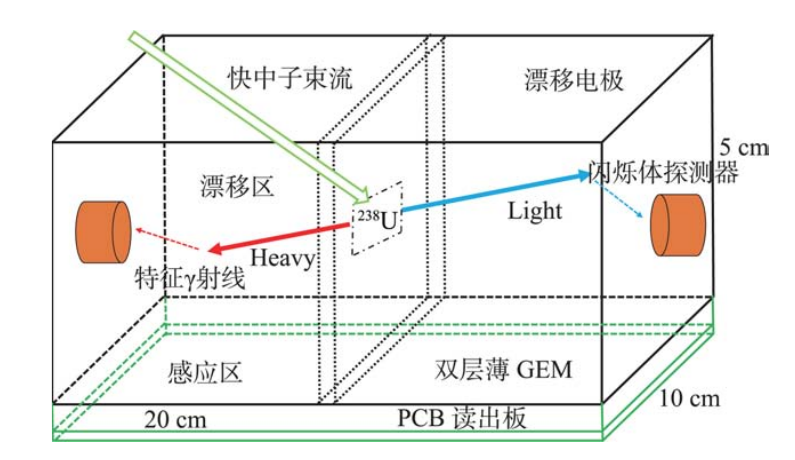
\includegraphics[width=0.7\textwidth]{figures/GEM-TPC.png}
    \caption{基于 GEM 工艺的 fTPC 探测系统\cite{魏康2019基于GEM工艺的裂变时间投影室中裂变碎片的讨论}}
    \label{fig_GEM-TPC}
\end{figure}

\begin{figure}[H]
    \centering
    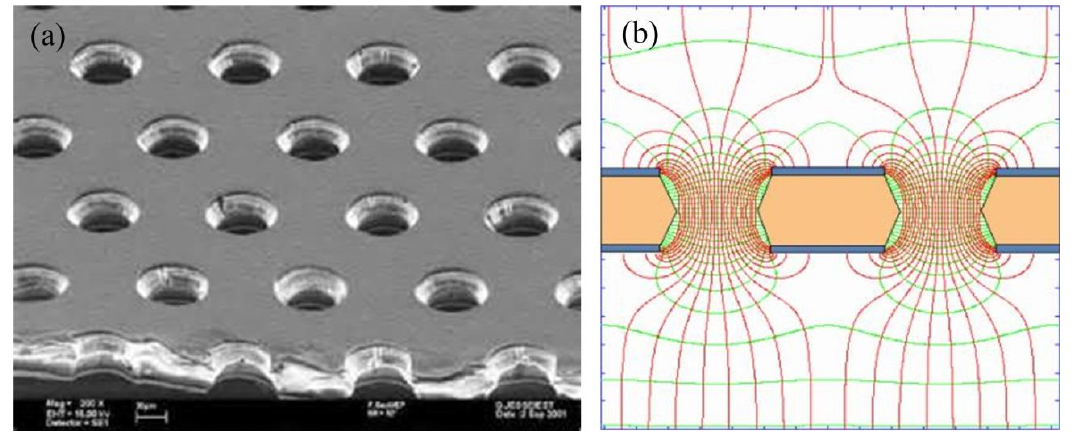
\includegraphics[width=0.7\textwidth]{figures/GEM.png}
    \caption{GEM 膜结构(a)和电场分布(b)}
    \label{fig_GEM}
\end{figure}


近年来,时间投影室技术因其在立体角、能量分辨以及多观测量关联测量等方面的显著优势而越来越多地应用于原子核裂变的实验研究中,对该方向的研究有很重要的推进作用。
目前由 M. Heffner 等人设计了高精度、高准确率的裂变事件投影室,用于主要锕系元素(U-235, U-238, Pu-239等)的裂变截面数据测量,其精度和准确率均好于 1\% \cite{heffner2014time}。
由 V. Geppert-Kleinrath 等人设计了用来测量锕系元素裂变碎片发射角度以及角各向异性(Angular Anisotropy)的裂变时间投影室,完成了对 U-235 在 160 keV 到 230 Mev 范围的中子诱发裂变的核数据测量,这是在该方向上的首次突破\cite{collaboration2019fission, hensle2020neutron}。
除此之外,结合使用深度学习的时间投影室也有越来越多的应用。例如 MicroBooNE Collaboration 基于液氩时间投影室(Liquid Argon Time Projection Chamber, LArTPC),应用卷积神经网络(Convolutional Neural Network, CNN)研究完成了对其产生的数据的算法研究。算法包括多粒子径迹图片的分类(Classification)、多粒子和中微子径迹图片中的空间定位(Localization)\cite{abratenko2020convolutional}。这些研究表明深度学习的卷积神经网络在此方向上大有潜力。
与上述各种传统实验方法相比,裂变时间投影室在各个方面都有较大的优势。与固体探测器相比,时间投影室的工作介质是气体,因此测量重离子能量时脉冲幅度损失较小,能量分辨率优势明显;与传统的弗里希屏电离室和以灯丝室和 PPAC 为代表的飞行时间探测器相比,时间投影室可以同时获得三维轨迹和全轨迹上能量沉积的详细信息,使得从能量损失中提取电荷信息的能力显著提高。

但上述成果大多用于不同条件下裂变截面、轻带电粒子及瞬发中子、$\gamma$的产额等方面的测量,对于裂变碎片的鉴别尚处于空白。
除此之外,目前对于裂变碎片的径迹重建仍然基于经典的离子能损理论,导致对重离子的核电荷数 的分析提取存在理论局限,尚未充分发挥时间投影室详细测量全径迹能量沉积行为的全部优势\cite{魏康2019基于GEM工艺的裂变时间投影室中裂变碎片的讨论}。
此外重离子碎片径迹末端核-核碰撞明显,导致径迹偏离原有的运动方向,如果将径迹简单地拟合为直线估算其能损无法准确处理这种非线性效应。

因此,本论文针对上述局限,提出借助人工神经网络算法不依赖于具体数学表达形式的独特优势,建立全新的裂变碎片径迹分析技术。






\section{论文工作的主要内容}
第一章是绪论部分,首先介绍了论文研究背景。尽管自原子核裂变发现 70 多年以来,人们一直在不断地进行研究,但是核裂变深层次地物理学仍然存在许多悬而未决的问题。在实际应用领域,已经完成了对裂变截面的高精度、高准确率的测量。并且还通过结合使用人工神经网络,完成了对时间投影室生成的径迹图片中的粒子的分类以及空间定位。但是目前对于裂变碎片的鉴别分类已经处于空白期,因此本论文借助深度学习人工神经网络,建立单核素径迹分类网络模型。


第二章从模拟计算产生的 U-235 裂变碎片事件数据出发。U-235 裂变碎片事件数据使用 fortran 的 fissionlib 计算 1MeV 中子轰击 U-235 后的产物分布,共生成 200000 例事件。
之后统计 200000 例裂变事件中的核素,使用 SRIM 生成每一个核素的重离子能损表。
最后使用 Garfield++ 调用 SRIM 的重离子能损表估算每一个裂变碎片在时间投影室内的径迹信息,完成裂变碎片的在时间投影室内的二维重建和三维径迹重建。

第三章基于第二章径迹重建产生的径迹数据,可以很容易地将生成的径迹数据转化为图像。因此,卷积神经网络(Convolutional Neural Network,CNN)自然非常适合这类图像数据的建模和训练。本论文使用已有的 CNN 神经网络模型,即使用迁移学习(Transfer Learning)建立人工神经网络模型。本论文中人工神经网络模型的输入是生成的径迹图像数据,输出是核素的核电荷数,模型使用的是 ResNet。结果表明,通过对预训练模型进行微调,显着地减少了训练时间。

第四章概括了全文的工作内容,总结了创新点并且展望了后续可能的优化。









\chapter{基于裂变时间投影室的径迹重建}
\section{时间投影室的工作原理}
David Nygren 在 1970 年代后期发明的时间投影室(Time Projection Chamber, TPC)是现在许多粒子和核物理实验中带电粒子径迹分析的基础\cite{nygren1978time}。
最初设计的时间投影室,可以允许在电子-正负电子对撞机上完全重建多达 20 个粒子的事件。
时间投影室是一种粒子检测器,能够对通过检测器介质传播的带电粒子进行完整的三维重建,同时可以准确测量粒子的电离能力。

时间投影室(见图 \ref{fig_GEM-TPC})一般包括四个组成部分\cite{闫洋洋2018用于高精度裂变截面测量的时间投影室, 魏康2019基于GEM工艺的裂变时间投影室中裂变碎片的讨论}:

(1)室腔(Chamber)本体。室腔本体为时间投影室的灵敏体积部分,其中充满了工作气体,待测粒子在其中漂移时损失能量,之后被时间投影室检测到;

(2)漂移电极。漂移电极接负高压,给时间投影室提供电场,这样粒子在漂移时产生的次级电子就能在漂移电场的作用下向 PCB 读出板方向漂移;

(3)场笼。场笼为时间投影室提供均匀电场。

(4)倍增元件和 PCB 读出板。倍增原件用来放大信号,从而可以避免时间投影室中信号较小的问题。现在常用的倍增元件有气体电子倍增器(GEM)和 Micromegas。读出板用来记录电子信号,这是径迹二维重建的基础。

\begin{figure}[H]
    \centering
    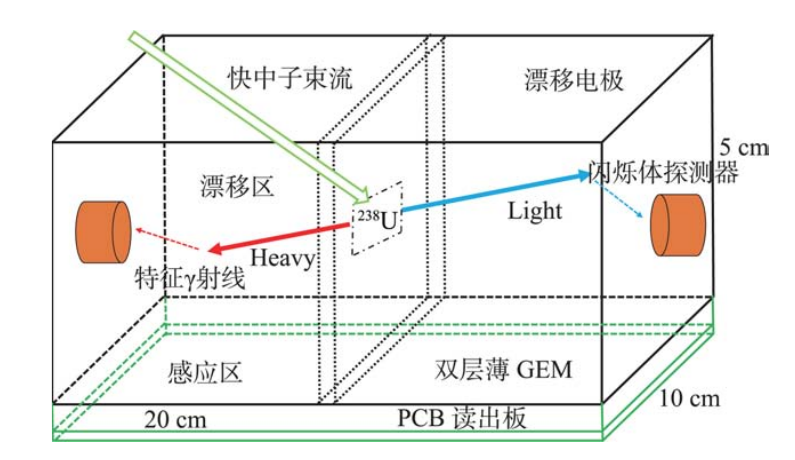
\includegraphics[width=0.7\textwidth]{figures/GEM-TPC.png}
    \caption{基于 GEM 工艺的 fTPC 探测系统\cite{魏康2019基于GEM工艺的裂变时间投影室中裂变碎片的讨论}}
    \label{fig_GEM-TPC}
\end{figure}


% 在时间投影室中,均匀电场作用下,带电粒子穿过室腔时会沿着漂移轨迹上产生电子/离子对,电子在漂移区均匀电场作用下向读出板上移动,之后通过记录读出板上的信号幅度和到达时间,就可以实现粒子轨迹的完整 3D 测量。

时间投影室具体的探测过程如下:

入射中子飞入时间投影室室腔,轰击在裂变靶材料上,然后引起原子核裂变,产生两个较轻质量的裂变碎片。根据动量守恒,裂变碎片相背飞出,进入两侧的漂移区内,在漂移过程中不断引起气体的电离,产生径迹。电离出的电子在匀场电场的作用下以近乎不变的速度向 PCB 读出板移动,经过气体电子倍增器放大信号之后被 PCB 读出电极收集。之后通过读出电极的位置和信号大小就可以测量碎片径迹在读出板上投影的位置(xz 坐标,二维径迹重建的基础),通过电子信号的持续时间测量径迹在竖直方向的位置(y 坐标,三维径迹重建的基础)\cite{魏康2019基于GEM工艺的裂变时间投影室中裂变碎片的讨论}。





\section{时间投影室的物理参数}
本论文的裂变时间投影室是基于兰州大学张毅等人研发的时间投影室\cite{魏康2019基于GEM工艺的裂变时间投影室中裂变碎片的讨论}。

物理尺寸:
如图 \ref{fig_GEM-TPC} 所示,裂变时间投影室的核心气体室腔的尺寸为 20x10x5 cm,分别代表 x,z,y 坐标。

工作气体:工作气体由 95\% 的氩气和 5\% 的异丁烷混合气体组成\cite{魏康2019基于GEM工艺的裂变时间投影室中裂变碎片的讨论}。

电压:漂移电极上接 6kV 左右的负高压,从而保证漂移区的电场强度为 1kV/cm 左右。

时间投影室的物理参数以及模拟所需的参数见表 \ref{tbl_TPC_parameters}。

\begin{table}[H]
    \centering
    \caption{裂变 TPC 模拟参数}
    \begin{tabular}{cc} % 控制表格的格式,可以是l,c,r
    \toprule
    物理对象& 参数 \\
    \midrule
    大气压 & 0.3 ATM \\
    温度 & 293.15 K \\
    工作气体 & 95\% Ar + 5\% iC4H10 \\
    裂变时间投影室 x 长度 & 20 cm \\
    裂变时间投影室 z 长度 & 10 cm \\
    裂变时间投影室 y 长度 & 5 cm \\
    漂移电场 & 1000 V/cm \\
    读出板读出电极形状 & 正方形 \\
    \bottomrule
    \end{tabular}
    \label{tbl_TPC_parameters}
\end{table}







\section{模拟裂变时间投影室}
\subsection{模拟软件介绍}
对裂变碎片事件的径迹重建采用了 Garfield++、SRIM、Geant4 和 ROOT等模拟软件,其中 Garfield++ 是径迹重建的核心软件。

Geant4 是由欧洲核子研究组织(CERN)使用 C++ 开发的软件包,用于模拟粒子在物质中输运的物理过程。Geant4 分为许多模块,分别负责处理几何跟踪、探测器响应、运行管理、可视化和用户界面。对许多物理模拟来说,这意味可以在实现细节上花费较少时间,使得研究者可以立刻着手从事模拟工作中重要的方面。Geant4 由于具有良好的通用性和扩展能力,在涉及微观粒子与物质相互作用的诸多领域获得了广泛应用。

ROOT 是 CERN 开发的面向对象的程序和库。它最初是为粒子物理数据分析而设计的,并且包含该领域特定的一些功能,但也用于其他应用程序,例如天文学和数据挖掘。每天,成千上万的物理学家使用 ROOT 应用程序分析其数据或执行模拟。ROOT 是使用 C++ 实现的,但是它也提供了一组绑定,以便与现有语言(例如Python和R)无缝集成,所以使用 ROOT 用来数据分析非常地方便。

SRIM 是核物理、粒子物理相关专业常用的一个软件,顾名思义,即计算离子在物质中的能量损失(即 dE/dx)和射程。在 SRIM 中,对所有处于移动中的原子,都统称为离子。

Garfield++ 是用 C++ 实现的面向对象的程序和库,用于模拟气体探测器中电子和阳离子与气体中原子的相互作用过程,并且可以计算电子在气体中扩散和漂移的相关参数,用于辅助探测器的优化设计。Garfield++ 还包括许多用于可视化目的的类,例如用于绘制电子漂移曲线、绘制静电势能的轮廓图和检查检测器的布局。这些类广泛依赖于 ROOT 框架。除此之外,Garfield++ 还依赖于 Geant4。

Garfield++ 的代码开源公布在 GitLab 上,如果你想 build Garfiled++ 或者是 build 基于 Garfield++ 的应用,你需要安装并配置好下列软件\cite{schindler2019garfield}:

\begin{itemize}
    \item ROOT
    \item 与 编译 ROOT 兼容的 C++ 编译器
    \item GSL (GNU Scientific Library)
    \item CMake (3.9 或者后续版本)
    \item Fortran 编译器
\end{itemize}




\subsection{模拟流程}
(1)生成裂变事件。本论文基于的是使用 Fortran 的 fissionlib 生成的 1MeV 中子轰击 U-235 后核裂变的产物分布,共 200000 例事件,每个事件包含裂变碎片的核素种类、能量、动量方向以及碎片的激发态能量等信息。见图 \ref{fig_U_235_events};

\begin{figure}[H]
    \centering
    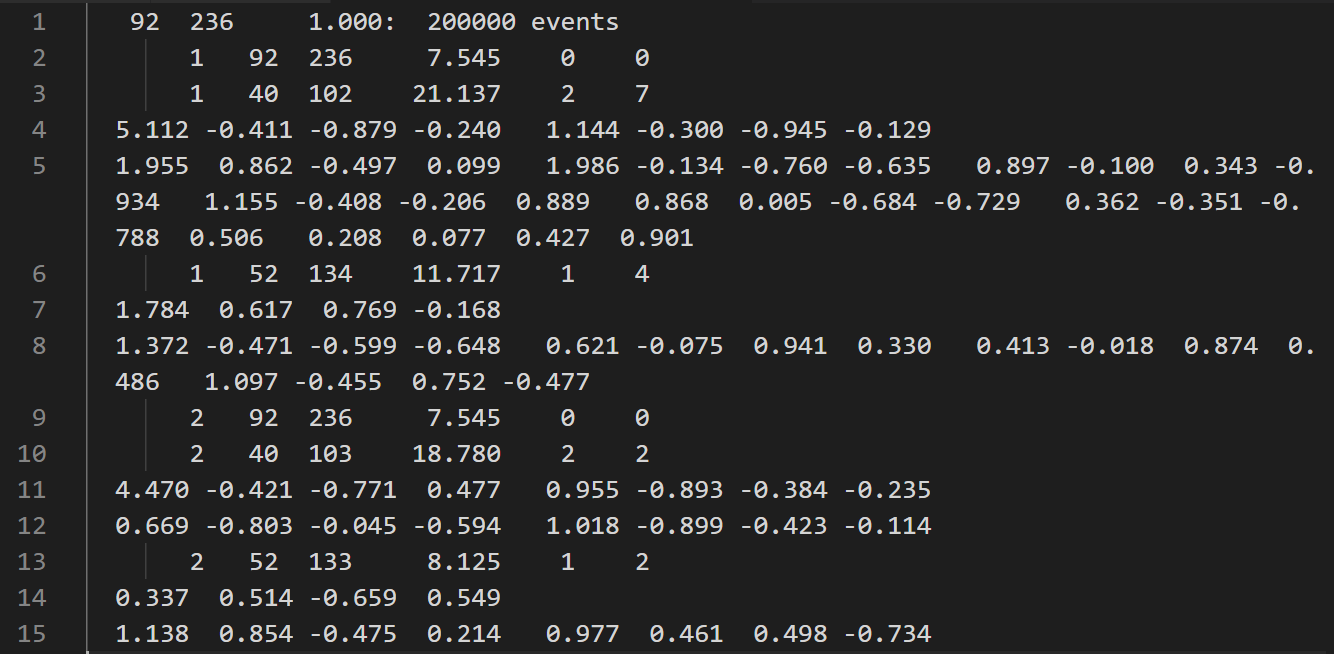
\includegraphics[width=0.7\textwidth]{figures/U-235-events.png}
    \caption{模拟的 U-235 前二个裂变事件}
    \label{fig_U_235_events}
\end{figure}

(2)统计 U-235 裂变事件信息,根据裂变事件中核素的出现次数和能量大小排序。见图 \ref{fig_statistics};

\begin{figure}[H]
    \centering
    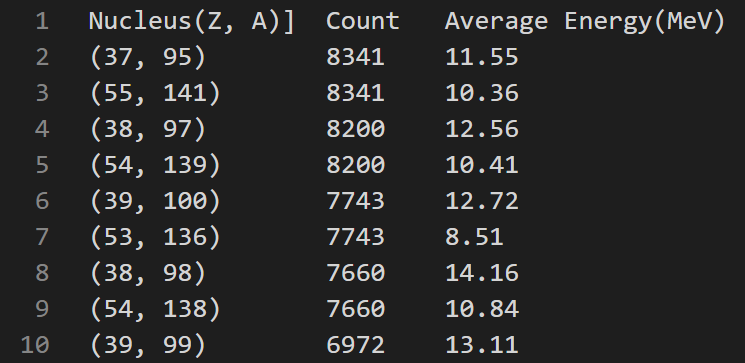
\includegraphics[width=0.7\textwidth]{figures/statistics.png}
    \caption{模拟的 U-235 裂变事件的统计}
    \label{fig_statistics}
\end{figure}

(3)根据(2)中得到的统计数据,选取出现频率高和能量大的裂变碎片核素,使用 SRIM 软件模拟生成对应的重离子能损数据表,其中包含带电离子在介质中的射程以及离子能损数据\cite{魏康2019基于GEM工艺的裂变时间投影室中裂变碎片的讨论, ziegler2010srim};

(4)使用 Garfield++ 下的 GasFile/generate.C 程序模拟生成裂变时间投影室的工作气体文件。生成的气体文件中参数有电子在工作气体中的漂移速度、吸附系数和扩散系数\cite{闫洋洋2018用于高精度裂变截面测量的时间投影室}。对于本论文基于的裂变时间投影室,在 GasFile/generate.C 程序中设定压力为 0.3 个大气压,温度为 293.15 K,工作气体为 95\% 的 Ar 和 5\% 的 iC4H10,其他参数保持默认值;

(5)然后以 Garfield++ 下的 Srim/srim.C 为模板,完成对裂变时间投影室的模拟。在 Srim/srim.C 中设定裂变事件投影室的的各个参数(具体参数见表 \ref{tbl_TPC_parameters}),并且在 Srim/srim.C 中代入(4)中生成的气体文件。到此已经完成了对裂变时间投影室物理结构的模拟。

(6)最后根据(2)中得到的统计数据,优先选取出现频率高和能量大的裂变碎片核素进行模拟。对于每一个核素,运行 srim.C 程序,代入(3)中生成的对应核素的重离子能损表、裂变碎片核素的能量、随机生成的三维方向矢量,从而使 Garfield++ 调用 SRIM 的重离子能损数据表估算每一个裂变碎片在时间投影室内的径迹信息,获得每一个事件在读出电极上的信号以及裂变碎片的停止位置。生成的数据见图 \ref{fig_output}。

\begin{figure}[H]
    \centering
    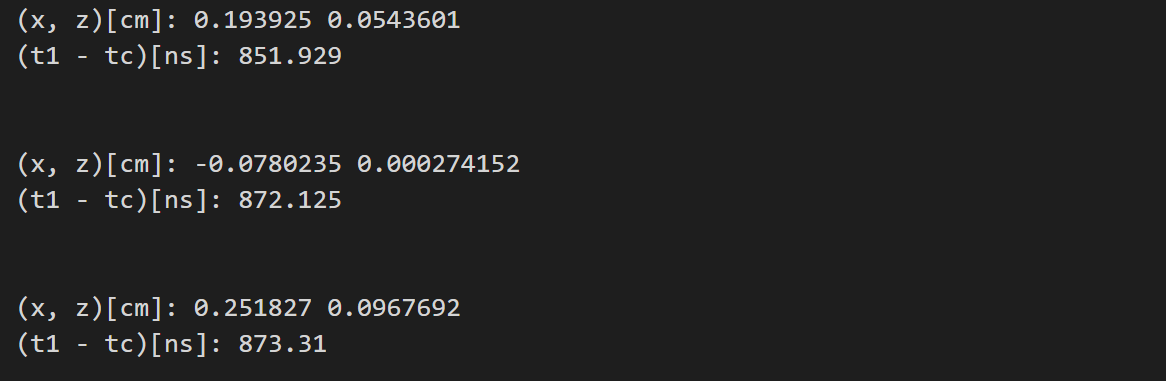
\includegraphics[width=0.7\textwidth]{figures/output.png}
    \caption{裂变时间投影室模拟的径迹数据}
    \label{fig_output}
\end{figure}




\section{数据分析和处理}
\subsection{二维径迹重建}
\label{sub:二维径迹重建}
如图 \ref{fig_output} 所示,对裂变时间投影室的模拟已经生成了各个电子在读出电极上的信号(x, z 坐标)以及电子到达读出电极上的时间。那么,根据各个电子的 x, z 坐标就可以完成模拟数据的径迹重建(见图 \ref{fig_track_2d_1})。

\begin{figure}[H]
	\centering
	\subfloat[37N95]{
        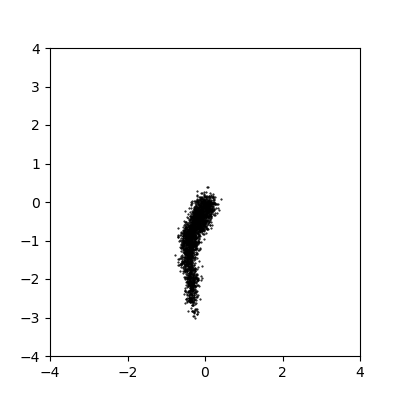
\includegraphics[width=0.3\textwidth]{figures/0.00236_-0.4095_0.91231.out_all_electrons.png}
    }
	\subfloat[37N95]{
        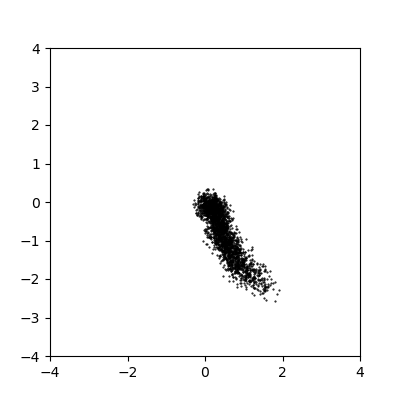
\includegraphics[width=0.3\textwidth]{figures/0.571_0.48881_0.65957.out_all_electrons.png}
    }
	\subfloat[37N95]{
        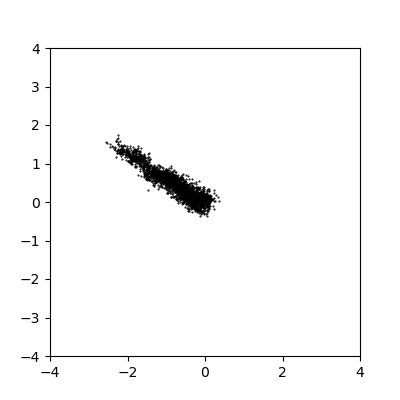
\includegraphics[width=0.3\textwidth]{figures/-0.7673_-0.39935_-0.50177.out_all_electrons.png}
    }\\	
    \caption{二维径迹图 1}
    \label{fig_track_2d_1}
\end{figure}

裂变时间投影室的读出板的尺寸是 20x10 cm,图 \ref{fig_output} 中得出的数据实际上是得不到的。因为读出板由多个读出电极组成,所以实际上我们只能得出每个电子对应的读出电极的坐标,为整数,而不是图 \ref{fig_output} 中的“精确坐标”。
如果将读出板中每一个读出电极的形状假设为正方形,并将图 \ref{fig_output} 中电子的坐标转化为读出电极的坐标,那么可以得到实际的径迹图像(见图 \ref{fig_track_2d_2})。

\begin{figure}[H]
	\centering
	\subfloat[37N95]{
        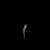
\includegraphics[width=0.3\textwidth]{figures/0.00236_-0.4095_0.91231.out_all_electrodes_double.png}
    }
	\subfloat[37N95]{
        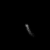
\includegraphics[width=0.3\textwidth]{figures/0.571_0.48881_0.65957.out_all_electrodes_double.png}
    }
	\subfloat[37N95]{
        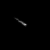
\includegraphics[width=0.3\textwidth]{figures/-0.7673_-0.39935_-0.50177.out_all_electrodes_double.png}
    }\\	
    \caption{二维径迹图 2}
    \label{fig_track_2d_2}
\end{figure}

上图中每一个像素所在的坐标对应了读出板上读出电极的坐标,像素值代表了对应读出电极上接受到的电子的数目(经过统计,电子数不会超出像素值的范围)。像素值的范围是 0-255,0 是纯黑色,255 是纯白色。






\subsection{三维径迹重建}
三维径迹重建需要计算 y 方向的坐标。对于三维径迹重建,由于裂变时间投影室中的电场可以近似为均匀电场,那么同样可以假设电子在裂变时间投影室中漂移的速度保持恒定,从而电子的 y 方向的数值就等于其到达读出板上的时间乘以它的漂移速度。

漂移速度可以通过 Garfield++ 下的 GasFile/read.C 程序模拟计算产生(需要使用前面生成的气体文件)。模拟产生的漂移速度如图 \ref{fig_drift_velocity}。
经过计算,裂变时间投影室中的漂移速度约等于 2.71E-3 cm/ns。最后,将每个电子到达读出电极上的时间乘以漂移速度即得到 y 方向的数值,从而完成了三维径迹重建。

\begin{figure}[H]
    \centering
    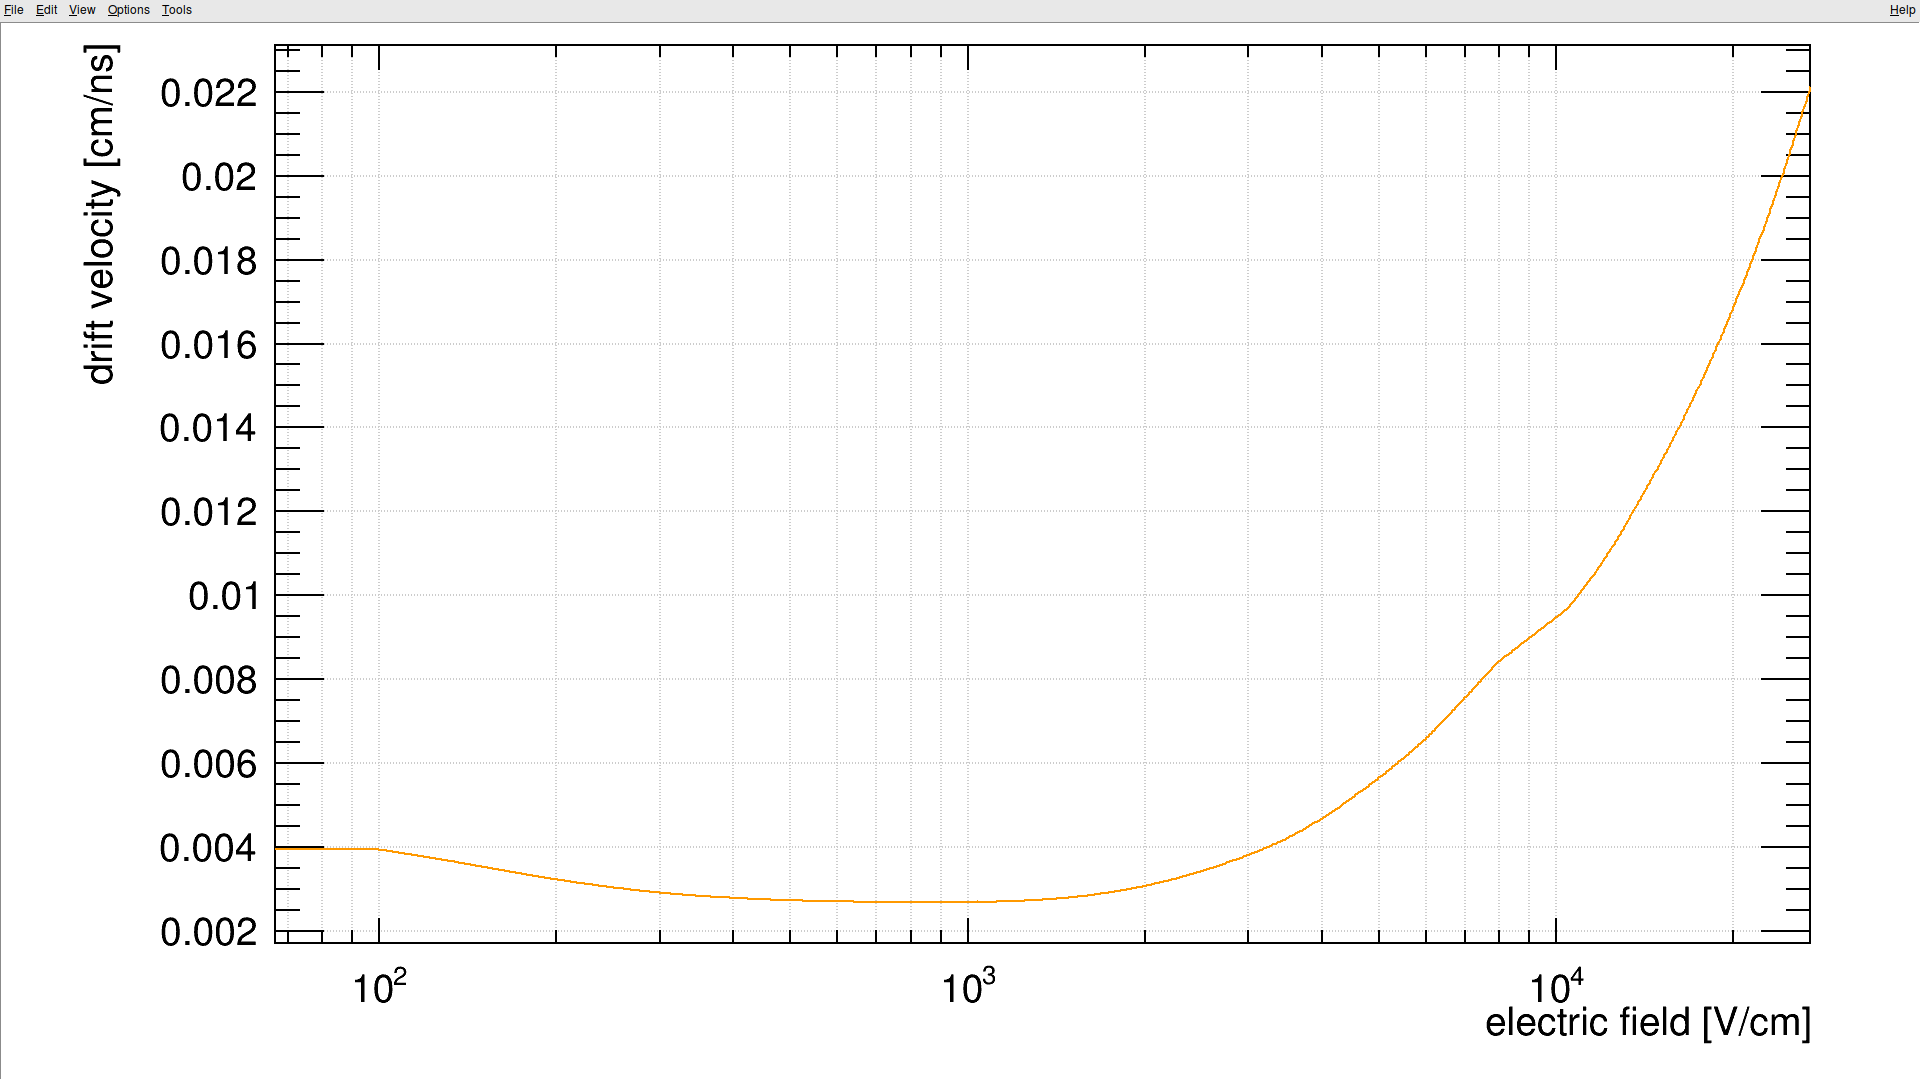
\includegraphics[width=0.8\textwidth]{figures/drift_velocity.png}
    \caption{漂移速度图}
    \label{fig_drift_velocity}
\end{figure}



\section{小结}
本章从使用 fissionlib 生成的 1MeV 中子轰击 U-235 模拟产生的 200000 个裂变事件出发,借助 Garfield++(及其依赖的 Geant4 和 ROOT)和 Srim,模拟了裂变时间投影室以及裂变碎片在室腔内的漂移,从而产生径迹信息,径迹信息包含电子在读出板上的坐标以及电子到达读出板上的时间等信息。
借助这些径迹信息以及利用 Garfield++ 计算出的漂移速度,完成了径迹的二维重建和三维重建。













\chapter{基于人工神经网络的裂变事件分类模型}
\section{机器学习介绍}
机器学习是实现人工智能的方法之一。机器学习有三类,分别是无监督学习、监督学习以及强化学习。
就像普通的编程方法一样,机器学习只不过是用来指定计算机执行一系列操作,然后完成某项任务。或者说,它也只不过是接受输入,执行某些任务,然后获得输出(见图 \ref{fig_input_output})。

\begin{figure}[H]
    \centering
    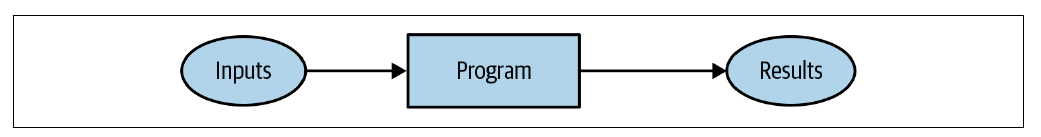
\includegraphics[width=0.8\textwidth]{figures/input_output.png}
    \caption{程序计算流程}
    \label{fig_input_output}
\end{figure}

但是机器学习的特点在于,对于某项任务,它不用(也不能)告诉计算机完成这项任务所需的每一个确切的步骤,而是将输入提供给机器学习模型,让机器学习模型自己“弄懂”如何解决这个问题(见图 \ref{fig_machine-learning})。

\begin{figure}[H]
    \centering
    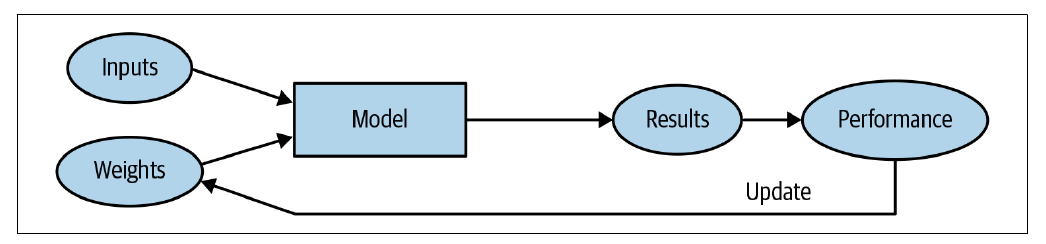
\includegraphics[width=0.8\textwidth]{figures/machine-learning.png}
    \caption{机器学习模型训练流程}
    \label{fig_machine-learning}
\end{figure}






\section{深度学习及人工神经网络介绍}
深度学习只是实现机器学习的算法之一,它最大的特点是使用了深度的人工神经网络。与机器学习类似,深度学习也是有无监督学习和监督学习之分的,并且不同模式的学习下建立的神经网络差别很大。常见的人工神经网络有卷积神经网络(CNN)、深度信念网络(DBN)和循环神经网络(RNN)等。

人工神经网络的特别和强大之处在于它的灵活性。万能近似定理(Universal Approximation Theorem)表明,只要找到合适的参数(weights),人工神经网络可以以任意准确度近似模拟出任何一个数学函数。

\begin{figure}[H]
    \centering
    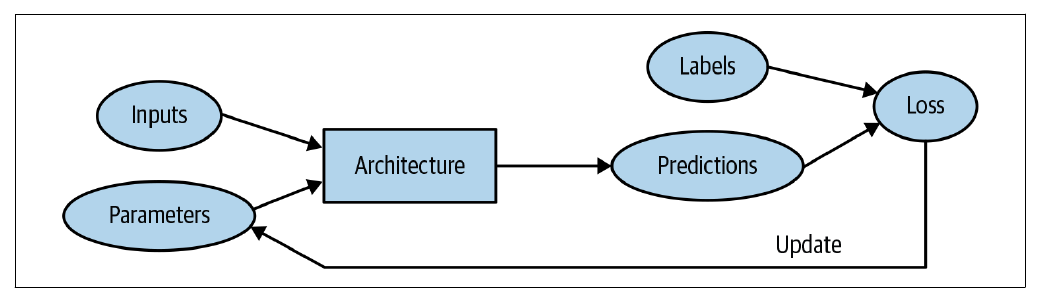
\includegraphics[width=0.8\textwidth]{figures/deep-learning.png}
    \caption{深度学习模型训练流程}
    \label{fig_deep-learning}
\end{figure}


这也就意味着尝试使用人工神经网络解决问题时,你只需要专注于找到合适的参数,剩下的工作可以交给网络模型,让它自己完成。而“找到合适的参数”这一任务也可以通过梯度下降算法(Stochastic Gradient Descent)帮我们自动完成。

\begin{figure}[H]
    \centering
    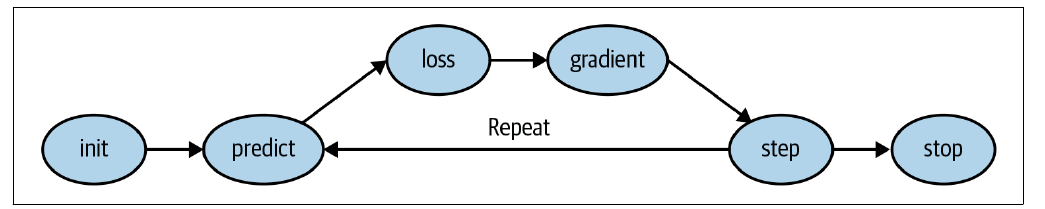
\includegraphics[width=0.8\textwidth]{figures/SGD.png}
    \caption{Stochastic Gradient Descent}
    \label{fig_SGD}
\end{figure}






\section{人工神经网络在核物理实验上的应用}
在核物理实验中,高能粒子碰撞产生的数据是巨量的,而这正好符合了深度学习对数据的“饥渴性”。而万能近似定理表明,只要找到合适的参数,人工神经网络可以以任意准确度近似模拟出任何一个数学函数。因此我们可以借助人工神经网络算法不依赖于具体数学表达形式的独特优势,将其应用于核物理实验研究中。

我们发现目前对于裂变碎片的径迹重建仍然基于经典的离子能损理论,导致对重离子的核电荷数的分析提取存在理论局限,尚未充分发挥时间投影室详细测量全径迹能量沉积行为的全部优势 \cite{魏康2019基于GEM工艺的裂变时间投影室中裂变碎片的讨论}。此外重离子碎片径迹末端核-核碰撞明显,导致径迹偏离原有的运动方向,如果将径迹简单地拟合为直线估算其能损无法准确处理这种非线性效应。在传统研究中,对于线性数据已经有很好的研究方法了。例如线性判别法(也叫 Fisher 判别法,Fisher's linear discriminant)\cite{fisher1936use},它对于鉴别线性可分的数据效果很好,但是对于非线性的样本则达不到合适的鉴别效果。而神经网络,基于它极其强大的灵活性,可以以任意精度模拟任意连续函数,因此对于非线性的问题,人工神经网络算法是非常合适的。

卷积神经网络(CNN)是人工神经网络的一个分支,它尤其擅长图像分析,例如图像分类、单个图像中物体定位等。通过对大量数据的学习,卷积神经网络能够在训练过程从图像中学习模式(pattern)和特征。卷积神经网络非常适合迁移学习(Transfer Learning)。也就是说,可以很容易地将训练于 A 数据集的网络模型应用于 B 数据集,并取得较好的结果。

目前,卷积神经网络在核物理实验上取得了丰富的成果,它越来越多地应用于中微子和高能物理实验中\cite{radovic2018machine, abratenko2020convolutional, abi2020neutrino, acciarri2017convolutional, racah2016revealing, aurisano2016convolutional, renner2017background}。例如 MicroBooNE Collaboration 基于液氩时间投影室(Liquid Argon Time Projection Chamber, LArTPC),应用卷积神经网络完成了对其产生的数据的算法研究。算法包括多粒子径迹图片的分类(Classification)、多粒子和中微子径迹图片中的空间定位(Localization)\cite{abratenko2020convolutional}。这些研究表明深度学习的卷积神经网络在此方向上大有潜力。

对于本论文,因为 Garfield++ 模拟时间投影室产生的径迹数据可以非常自然地转化为 2D 图像,所以借助卷积神经网络以及迁移学习可以实现数据的快速分析,并同时得到较好的准确度。




\section{建立神经网络模型}
\subsection{网络参数}
神经网络训练流程如下图。

\begin{figure}[H]
    \centering
    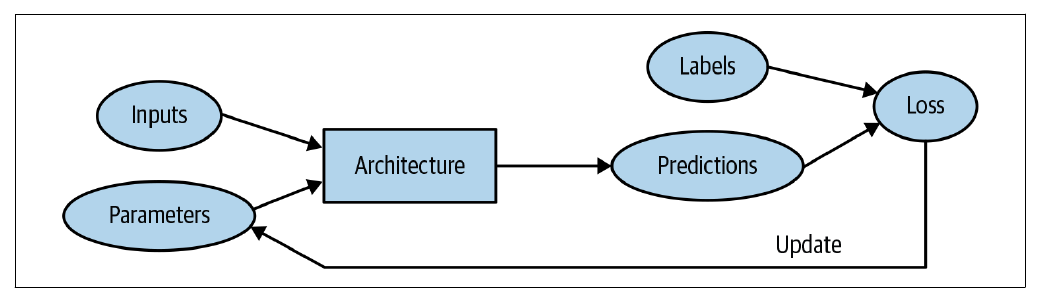
\includegraphics[width=0.8\textwidth]{figures/deep-learning.png}
    \caption{深度学习模型训练流程}
    \label{fig_deep-learning}
\end{figure}


本论文使用的迁移学习,因此建立神经网路模型时网络参数的侧重点在于 Inputs,Prediction 以及 Architecture。对于我们的网络模型,Inputs 即我们在 \ref{sub:二维径迹重建}中生成的径迹图像。径迹图像的每一个像素所在的坐标代表了一个特定读出电极的坐标,像素值代表了对应读出电极上的电子数目。Predictions 代表我们的网络模型的输出,在该模型中,输出是图片中裂变碎片径迹所代表的核素种类。Architecture,即网络架构,是模型的核心。


\subsection{网络训练}
本论文使用了 fastai\cite{howard2020fastai} 建立人工神经网络模型。
fastai 是一个基于 PyTorch 的深度学习类库,为深度学习使用者提供高级抽象组件,这些组件可以快速轻松地提供标准深度学习领域中的最新结果,并为研究人员提供可以混合和匹配以构建的低级组件新方法。使用 fastai 的高阶抽象 API,我们可以极快速地完成人工神经网络的建模,但同时也不失灵活性。

使用 fastai 训练我们的裂变事件分类网络模型的核心代码如下:

(1)导入 fastai 以及相关的 CNN 类库
\begin{lstlisting}[language = python]
from fastbook import *
from torchvision.models import *

from fastai.vision import *
from fastai.vision.models import *
from fastai.vision.widgets import *
from fastai.vision.learner import model_meta
\end{lstlisting}

(2)创建神经网络数据集
\begin{lstlisting}[language = python]
img_dir = Path('PATH_TO_IMAGES')
tracks = DataBlock(
    blocks=(ImageBlock, CategoryBlock),
    get_items=get_image_files, 
    splitter=RandomSplitter(valid_pct=0.2, seed=474),
    get_y=get_img_Z)

dls = tracks.dataloaders(img_dir)
\end{lstlisting}


(3)神经网络训练
\begin{lstlisting}[language = python]
learn = cnn_learner(dls, YOUR_ARCHITECTURE, metrics=accuracy)
learn.fine_tune(10)
\end{lstlisting}




\subsubsection{网络架构(Architecture)的选择}
本论文测试了 CNN 下流行的架构,包括 ResNet, XResnet, DenseNet, VGG, SqueezeNet, ShuffleNet 等架构(见表 \ref{tbl_architectures})。


\begin{table}[H]
    \centering
    \caption{神经网络架构}
    \begin{tabular}{cc} % 控制表格的格式,可以是l,c,r
    \toprule
    架构名 & 具体参数 \\
    \midrule
    ResNet & Resnet18, Resnet34, Resnet50, Resnet102, Resnet152 \\
    XResnet & XResnet18, XResnet34, XResnet50, XResnet102, XResnet152 \\
    DenseNet & DensetNet121, DensetNet161, DensetNet169, DensetNet201 \\
    VGG & VGG11\_bn, VGG13\_bn, VGG16\_bn, VGG19\_bn \\
    SqueezeNet & squeezenet1\_0, squeezenet1\_1 \\
    ShuffleNet & shufflenet\_v2\_x0\_5, shufflenet\_v2\_x1\_0 \\
    \bottomrule
    \end{tabular}
    \label{tbl_architectures}
\end{table}



\subsubsection{训练结果}
目前最好可以同时对 6 种核素(39N100, 53N136, 37N95, 55N141, 40N102, 52N134)以不低于 99.5\% 的正确率完成分类。

\begin{figure}[H]
	\centering
	\subfloat[Accuray]{
        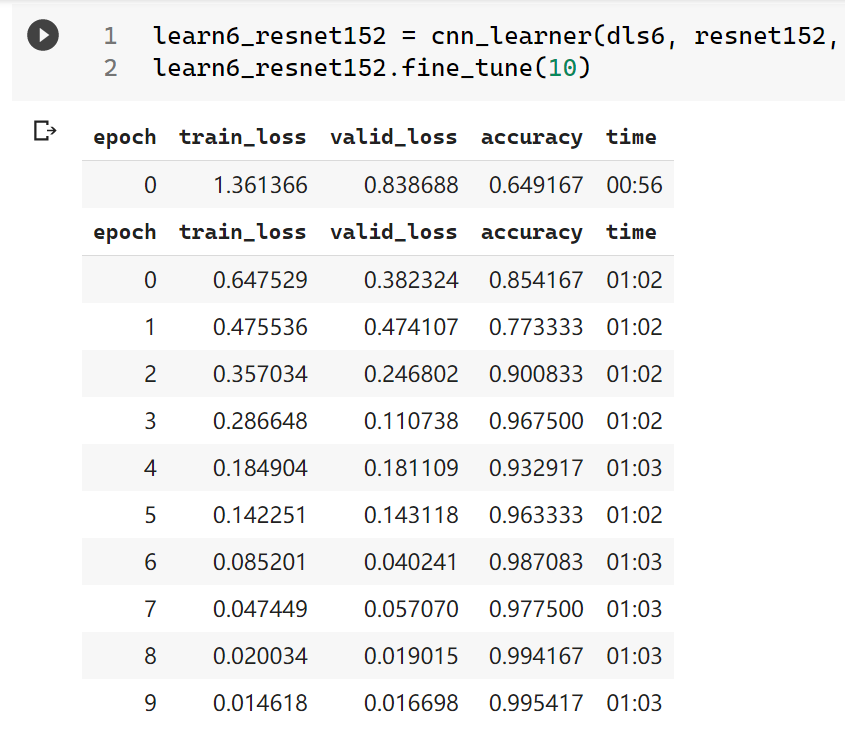
\includegraphics[width=0.5\textwidth]{figures/learn6-resnet152.png}
    }
	\subfloat[Loss]{
        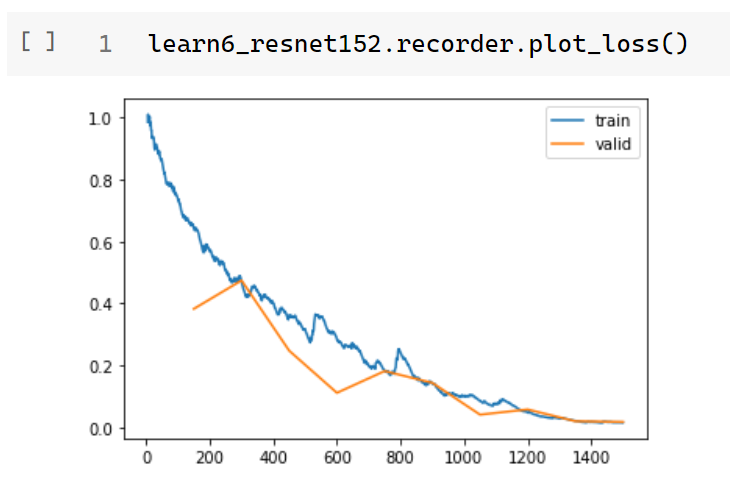
\includegraphics[width=0.5\textwidth]{figures/learn6-resnet152-loss.png}
    }\\	
    \caption{6 种核素训练结果(ResNet152)}
    \label{fig_learn6_resnet152}
\end{figure}


\begin{figure}[H]
	\centering
	\subfloat[Accuray]{
        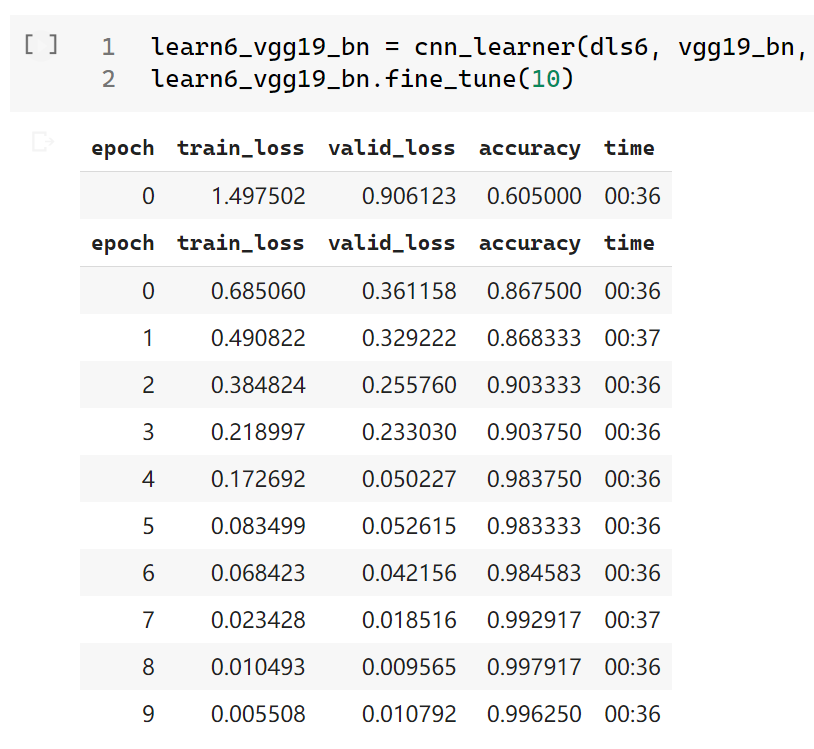
\includegraphics[width=0.5\textwidth]{figures/learn6-vgg19-bn.png}
    }
	\subfloat[Loss]{
        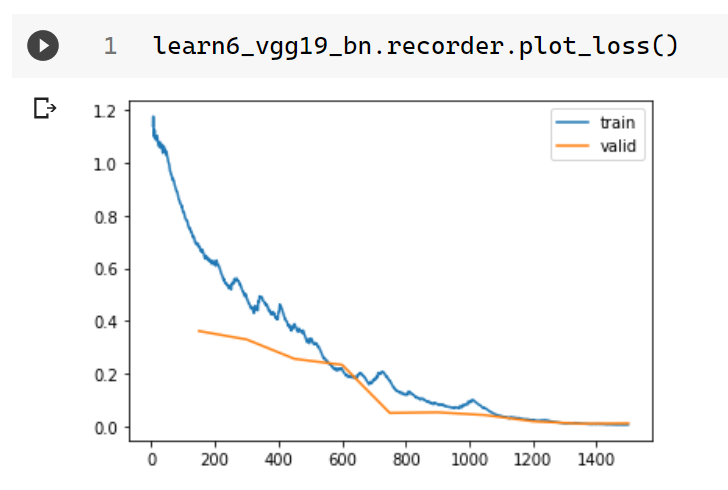
\includegraphics[width=0.5\textwidth]{figures/learn6-vgg19-bn-loss.png}
    }\\	
    \caption{6 种核素训练结果(VGG19\_bn)}
    \label{fig_learn6_vgg19-bn}
\end{figure}


除此之外,可以同时对 12 种核素(35N90, 36N92, 37N95, 38N97, 39N100, 40N102, 52N134, 53N136, 54N139, 55N141, 56N144, 57N146)以不低于 80\% 的正确率完成分类。

\begin{figure}[H]
	\centering
	\subfloat[Accuray]{
        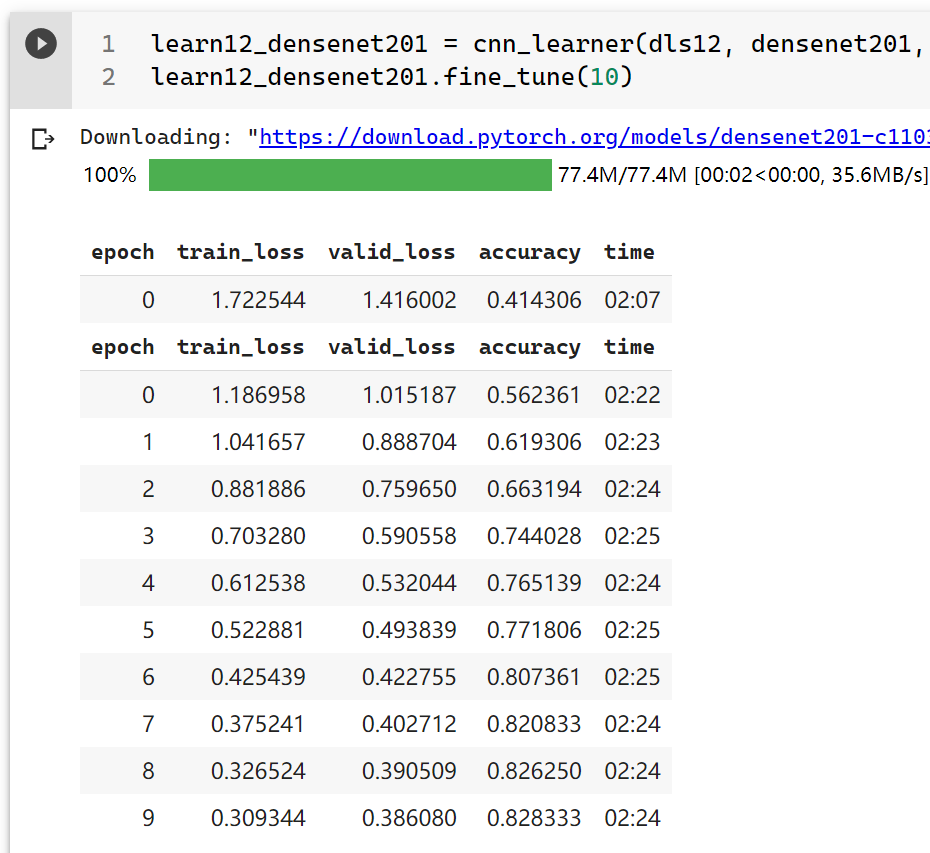
\includegraphics[width=0.5\textwidth]{figures/learn12-densenet201.png}
    }
	\subfloat[Loss]{
        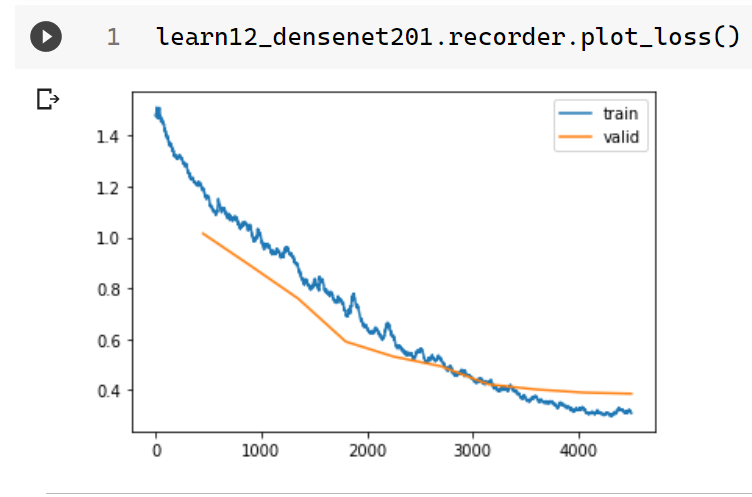
\includegraphics[width=0.5\textwidth]{figures/learn12-densenet201-loss.png}
    }\\	
    \caption{12 种核素训练结果(DenseNet201)}
    \label{fig_learn12-densenet201}
\end{figure}

\begin{figure}[H]
	\centering
	\subfloat[Accuray]{
        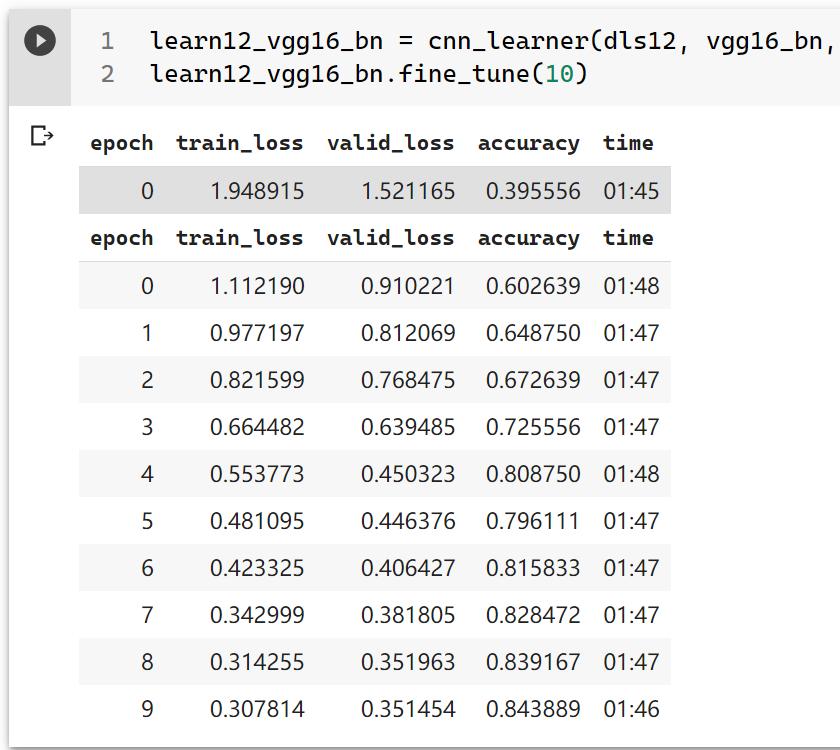
\includegraphics[width=0.5\textwidth]{figures/learn12-vgg16-bn.png}
    }
	\subfloat[Loss]{
        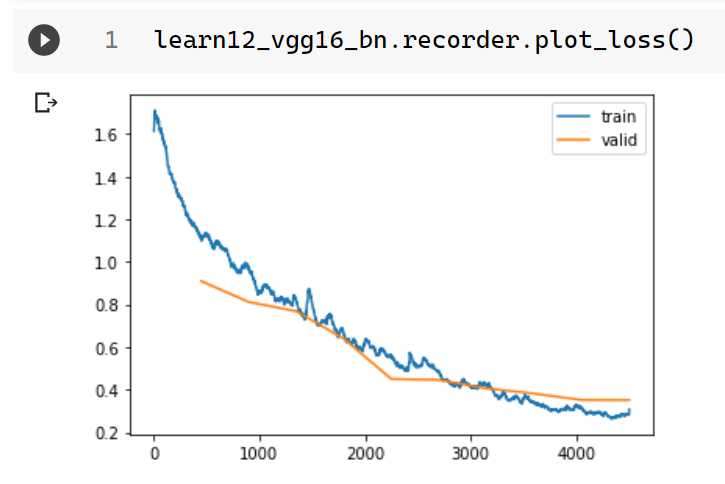
\includegraphics[width=0.5\textwidth]{figures/learn12-vgg16-bn-loss.png}
    }\\	
    \caption{12 种核素训练结果(VGG16\_bn)}
    \label{fig_learn12-vgg16-bn}
\end{figure}


本论文神经网络训练过程中使用了 ResNet, XResnet, DenseNet, VGG 等架构。经过统计,总体上 VGG 架构的训练结果最好,如上述表格中所示,对于 6 种核素的神经网络,使用 VGG 架构的模型在未过拟合(Over Fitting)之前可达到 99.8\% 的正确率,对于 12 种核素的神经网络,使用 VGG 架构的模型在未过拟合之前可达到 81.6\% 的正确率完成分类。ResNet, XResNet 以及 DenseNet 的训练结果比 VGG 稍差,6 种核素的正确率为 97\% 左右。SqueezeNet 和 ShuffleNet 架构的训练结果较差,不适合该模型。

除此之外,神经网络的层数对训练结果的正确率有影响,经过统计,神经网络层数越多,模型更容易过拟合,但是同时也能在过拟合之前达到更高的正确率。因此,扩大训练数据集的容量以及增加神经网络的层数可以提高模型的最终正确率。



\section{网络测试}
下面使用 6 种核素(39N100, 53N136, 37N95, 55N141, 40N102, 52N134)建立的模型对其他核素(见图 \ref{fig-other-nuclides})进行测试。


\begin{figure}[H]
    \centering
    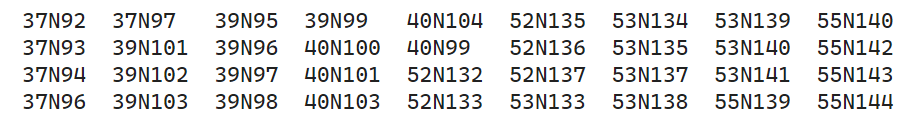
\includegraphics[width=0.8\textwidth]{figures/other-nuclides.png}
    \caption{测试的核素}
    \label{fig-other-nuclides}
\end{figure}

测试实例代码如图 \ref{fig-test-code}:

\begin{figure}[H]
    \centering
    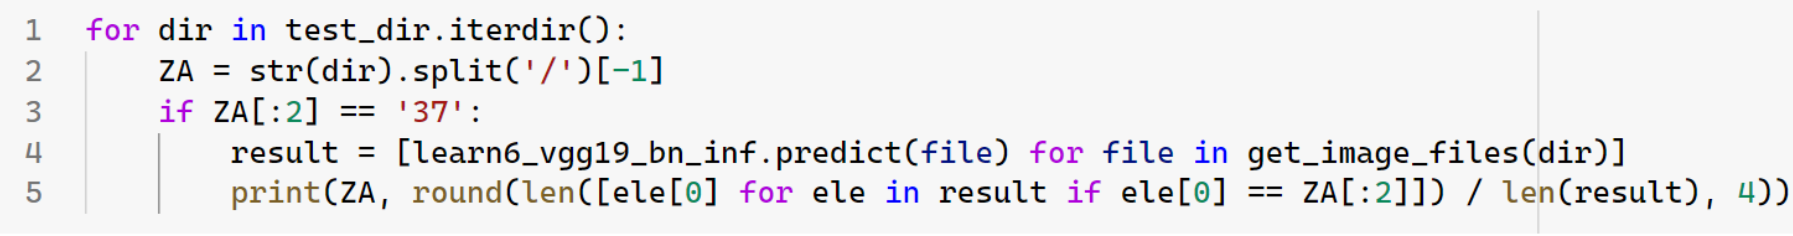
\includegraphics[width=1.0\textwidth]{figures/test-code.png}
    \caption{测试实例代码}
    \label{fig-test-code}
\end{figure}


结果如图 \ref{fig-test-output}。
数据表明,只用 6 种核素(39N100, 53N136, 37N95, 55N141, 40N102, 52N134)建立的模型,就可以对图 \ref{fig-other-nuclides} 完成较好的鉴别分类。在本神经网络模型中,对训练结果影响最大的是径迹图像中的电子数目或像素的数目。而电子数目对应的是能损(dE/dx),由于模型中并没有使用三维径迹计算能损(dE/dx)并把能损用于训练模型,这是本模型的不足之处,因为本模型对图 \ref{fig-test-output} 中某些核素的测试结果很差。

\begin{figure}[H]
	\centering
	\subfloat[37]{
        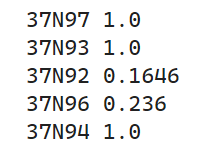
\includegraphics[width=0.2\textwidth]{figures/37-result.png}
    }
    \subfloat[39]{
        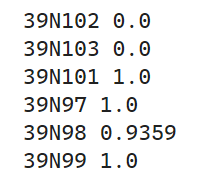
\includegraphics[width=0.2\textwidth]{figures/39-result.png}
    }
	\subfloat[40]{
        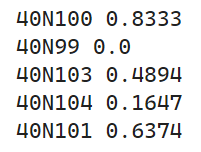
\includegraphics[width=0.2\textwidth]{figures/40-result.png}
    }\\	
    \subfloat[52]{
        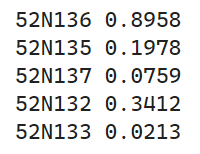
\includegraphics[width=0.2\textwidth]{figures/52-result.png}
    }
    \subfloat[53]{
        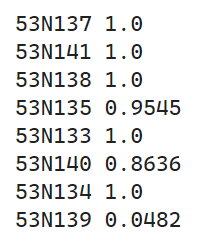
\includegraphics[width=0.2\textwidth]{figures/53-result.png}
    }
	\subfloat[55]{
        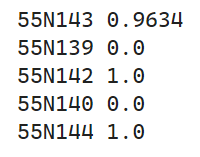
\includegraphics[width=0.2\textwidth]{figures/55-result.png}
    }\\	
    \caption{测试结果}
    \label{fig-test-output}
\end{figure}

图 \ref{fig-test-output} 中核素的概率指预测概率大于 0.5 的测试数据占总测试数据的比率。



\section{结果分析}
与传统的的核物理分析手段相比,基于人工神经网络的鉴别方法不需要借助具体数学表达形式,这是它的独特优势。本论文中的人工神经网络基于 fastai 高阶抽象 API 建立,建模建立以及数据分析速度非常快。在模型建议过程中只需要操心输入层,并且后续可以非常容易地将已建立的模型应用于新的环境,只需要更换输入层的数据集即可。

在建立人工神经网络模型中,数据的预处理毫无疑问是最重要的,它直接影响了后续的网络训练效果。对于本论文中人工神经网络模型的输入数据,它只包含了能量和射程信息。能量对应了 2D 径迹图片上的像素大小,射程对应了图片上黑色像素的范围。也正是因为输入层只包含能量和射程信息,网络模型能力才非常有限。实际上,除了上能量和射程信息外,还可以将粒子的能损(dE/dx)信息加入输入层,例如粒子的能损的最大值以及粒子能损的最大值出现在的位置等信息 \cite{闫洋洋2018用于高精度裂变截面测量的时间投影室},这样,后续的训练结果必然会更好。

不管怎样,随着神经网络编程技术的不断发展,学习神经网络编程绝对会变得越来越容易,高阶抽象的神经网络 API 会越来越多、越来越容易使用,预训练好的模型(Pretrained Model,用来迁移学习)也会越来越多面。因此只要有足够可用的数据并对其进行正确的数据处理,再结合使用迁移学习(Transfer Learning),使用别人已经训练好的模型,那么后续开发和研究速度将会变得极速。



\section{小结}
本章从第二章生成的二维径迹图像数据出发,将径迹图像数据作为人工神经网络模型的输入,调用 基于 PyTorch 的 fasti 高阶 API,使用 ResNet, XResnet, DenseNet, VGG, SqueezeNet, ShuffleNet 等 CNN 架构进行迁移学习,建立了裂变碎片径迹图像的分类模型。建立的网络模型可以同时对 6 种核素(39N100, 53N136, 37N95, 55N141, 40N102, 52N134)以不低于 99.5\% 的正确率完成鉴别分类。








\chapter{结论与展望}
\section{总结}
原子核裂变发现 70 多年以来,人们一直在不断地进行研究,但是核裂变深层次地物理学仍然存在许多悬而未决的问题。在实际应用领域,已经完成了对裂变截面的高精度、高准确率的测量。并且还通过结合使用人工神经网络,完成了对时间投影室生成的径迹图片中的粒子的分类以及空间定位。但是目前对于裂变碎片的鉴别分类已经处于空白期,因此本论文借助深度学习人工神经网络,建立单核素径迹分类网络模型。

本论文从模拟计算产生的 U-235 裂变碎片事件数据出发,使用 SRIM 生成每一个核素的重离子能损表,然后使用 Garfield++ 调用 SRIM 的重离子能损表估算每一个裂变碎片在时间投影室内的径迹信息,完成裂变碎片的在时间投影室内的二维重建和三维径迹重建。

之后使用 fastai,以二维径迹图像为输入数据,完成了裂变碎片径迹图像的鉴别分类。建立的网络模型最好可以同时对 6 种核素以不低于 99.5\% 的准确率完成核素分类,除此之还,还可以对 12 种核素以不低于 80\% 的正确率完成分类。



\section{展望}
生成人工神经网络的输入数据耗时巨大,由于时间限制,本论文只生成了 12 种核素的径迹数据,每个核素大约生成了 3000 份数据,后续通过增大数据量(单个核素径迹数、总核素数目)以及提高径迹数据精度可以提高模型的鉴别能力。除此之外,通过将粒子的能损(dE/dx)信息加入输入层,例如粒子的能损的最大值以及粒子能损的最大值出现在的位置等信息 \cite{闫洋洋2018用于高精度裂变截面测量的时间投影室},必然可以加强网络的训练效果。


%论文后部
\backmatter


%=======%
%引入参考文献文件
%=======%
\bibdatabase{bib/database}%bib文件名称 仅修改bib/ 后部分
\printbib
% \nocite{*} %显示数据库中有的,但是正文没有引用的文献



\Thanks
感谢张毅老师在这几个月期间对我不厌其烦地指导。我物理知识匮乏,所以一直在 QQ 上频繁地请教张毅老师,感谢张毅老师总能及时且详细准确地对我的问题给出解答,和张毅老师相处绝对是一件非常愉快且难忘的事。

感谢兰大学长在 GitHub 上提供的 latex 模板,让我能够不用操心论文的格式,只专注论文内容。

\end{document}
